\documentclass[12pt, a4paper]{article}
\usepackage[margin=1.0 in]{geometry}
\addtolength{\topmargin}{.25in}
\usepackage[utf8]{inputenc}  
\usepackage{amsmath}
\usepackage[danish]{babel}
\usepackage{calc}
\usepackage{array}
\usepackage{amssymb}
%\usepackage{tikz}
\usepackage{graphicx}
\newcommand{\HRule}{\rule{\linewidth}{0.5mm}}
\usepackage{hyperref}
\newcommand{\Green}{\tikz\draw[green,fill=green] (0,0) circle (1 ex);}
\newcommand{\Lime }{\tikz\draw[brown,fill=brown] (0,0) circle (1 ex);}
\newcommand{\Blue}{\tikz\draw[blue,fill=blue] (0,0) circle (1 ex);}
\newcommand{\Yellow}{\tikz\draw[yellow,fill=yellow] (0,0) circle (1 ex);}
\newcommand{\Red}{\tikz\draw[red,fill=red] (0,0) circle (1 ex);}
\renewcommand*\contentsname{Indholdsfortegnelse}
%\usepackage{cleveref}

%\crefformat{footnote}{#2\footnotemark[#1]#3}

\setlength\parindent{0pt}		% noindent through whole document
\usepackage[parfill]{parskip}	% extra linebreak on new paragraph
\begin{document}
\section*{Gruppeaflevering}
I denne opgave skulle vi arbejde med den deterministiske optimeringsalgoritme gradient descent, ved at fjerne støj fra et billede, der er et klassisk problem inden for billedbehandling.

\section*{Gradient billeder}
De to gradient-billeder er visualiseret, ud fra billedet uden støj, længere nede som Figur 1 (gradient-x) og Figur 2 (gradient-y).
Efter sammenligning, ses det tydeligt at Figur 1 er magen til (iii) fra ugesedlen og ligeledes Figur 2 er magen til figur (ii) fra ugesedlen.
Grunden til at y-x og x-y skyldes sandsynligvis ombytningen af de to gradienter, som vi fandt ud af til øvelsestimen.

\subsection*{Normen}
Normen der udregnet ud fra de to gradienter, er visualiseret nedenunder i Figur 3. Efter sammenligning, ses det tydeligt at Figur 3 er magen til (iii) fra ugesedlen.

\subsection*{Divergensen}
Divergensen beskriver forskellen på hver af de to gradient billeder, i forhold til hindanden og ligger disse sammen. Altså forskellen på pixels omkring den evaluerede pixel (indgangen i matrixen). Figur 4 ses divergensen, hvor kontrasten/forskellen mellem pixels i et punkt er illustreret.

\subsection*{Grafen til 5.5}
Grafen (Figur 5) opfører sig som forventet, idet at vi ser en tydelig reduktion af støjen, som bliver mindre og mindre for hver iteration og konvergerer mod et punkt, der ville være det originale billede.

\subsection*{Effekten af lambda}
Ved at gøre lambda mindre, bliver billedet mere ufokuseret/udtværet.\\
Ved at forstørre lambda, bliver billedet mere fokuseret, men mindre støjreduceret.

\subsection*{Konklusion}
Det har lykkedes os at lave et program, der indlæser et billeder og reducerer støjen på dette, ved brug af $gradient-descent$. Efterfølgende, ved at betragte Figur 5, ses det at ved omkring 20 iterationer af reduceringen, er optimeringen af billedet minimalt, at det ikke kan betale sig at køre flere end det. Figur 6 beskriver vores støj-reducerede billede og Figur 7 er det angivne billede med støj vi har skullet reducere.

\begin{figure}[H]
  \caption{Billede af Gradient-y}
  \centering
	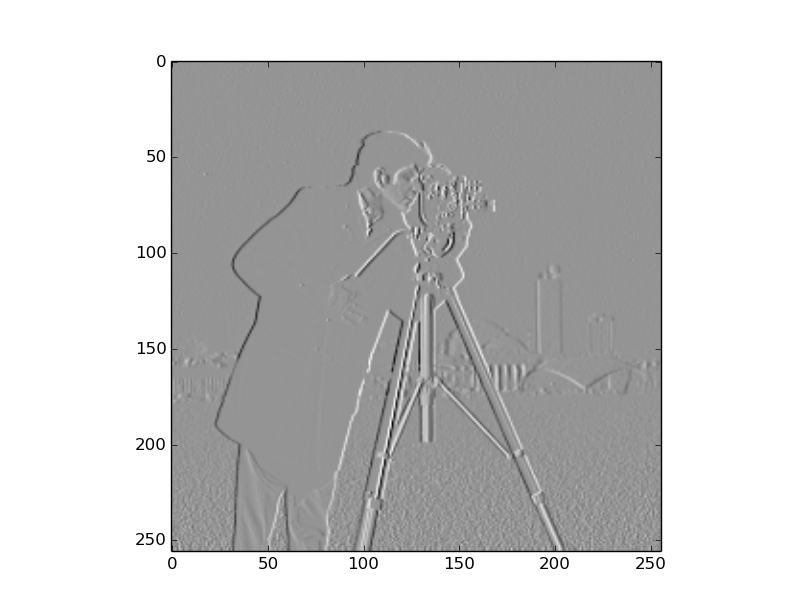
\includegraphics[scale=0.8]{grady}
\end{figure}
\begin{figure}[H]
  \caption{Billede af Gradient-x}
  \centering
	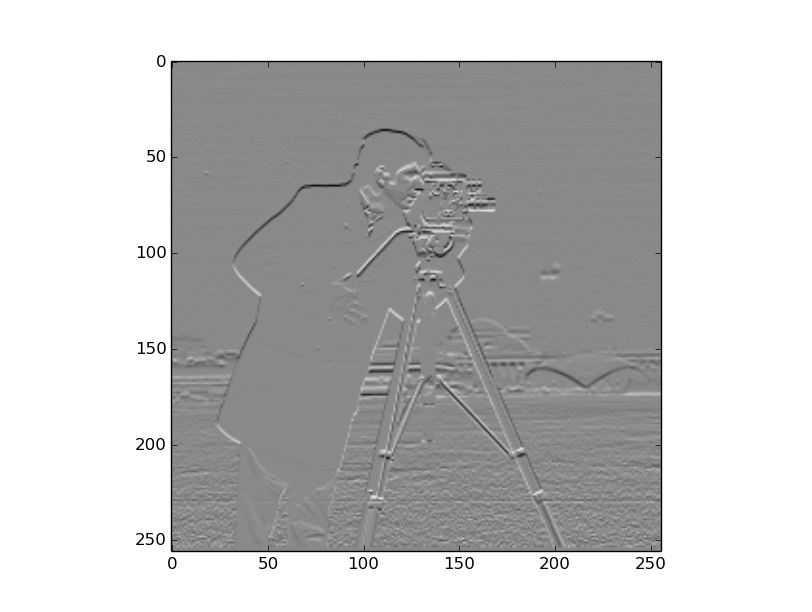
\includegraphics[scale=0.8]{gradx}
\end{figure}
\begin{figure}[H]
  \caption{Billede af Normen}
  \centering
	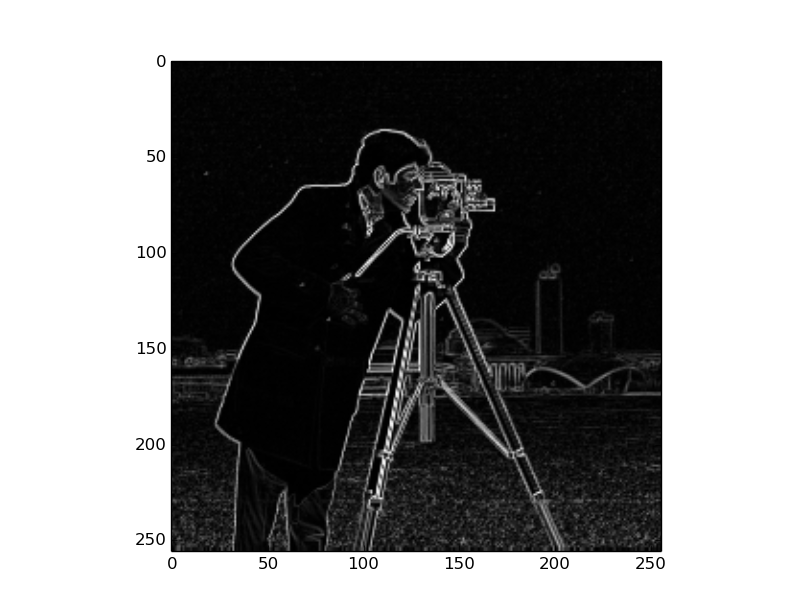
\includegraphics[scale=0.8]{norm}
\end{figure}
\begin{figure}[H]
  \caption{Billede af Divergensen}
  \centering
	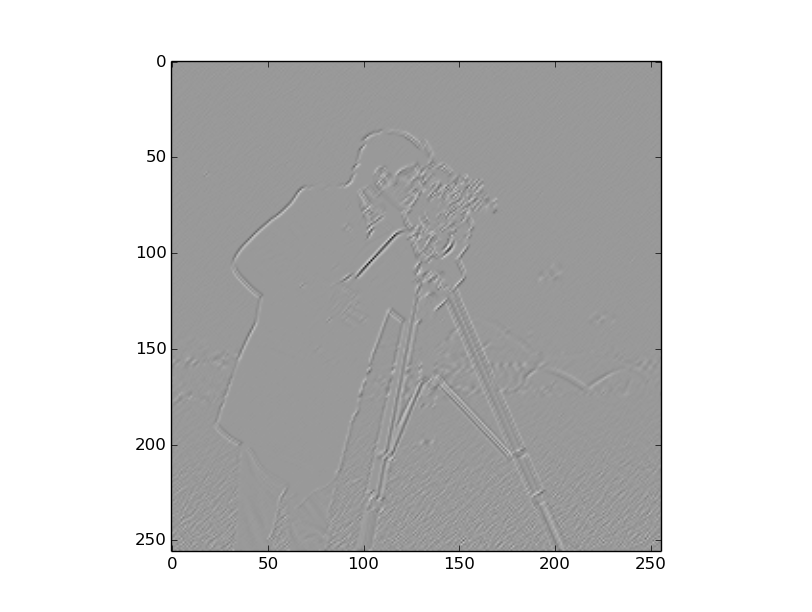
\includegraphics[scale=0.8]{diver}
\end{figure}
\begin{figure}[H]
  \caption{Billede af Støj-reduceringen}
  \centering
	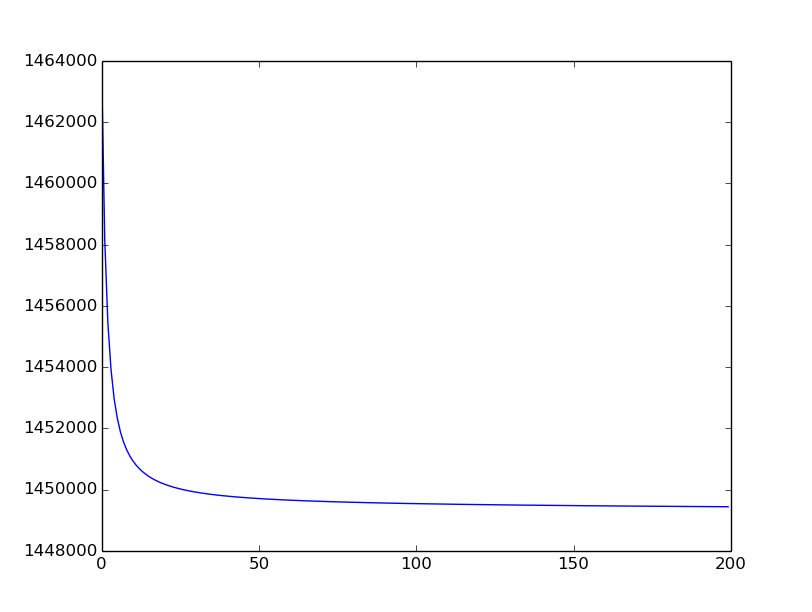
\includegraphics[scale=0.8]{energi}
\end{figure}
\begin{figure}[H]
  \caption{Billede med støj}
  \centering
	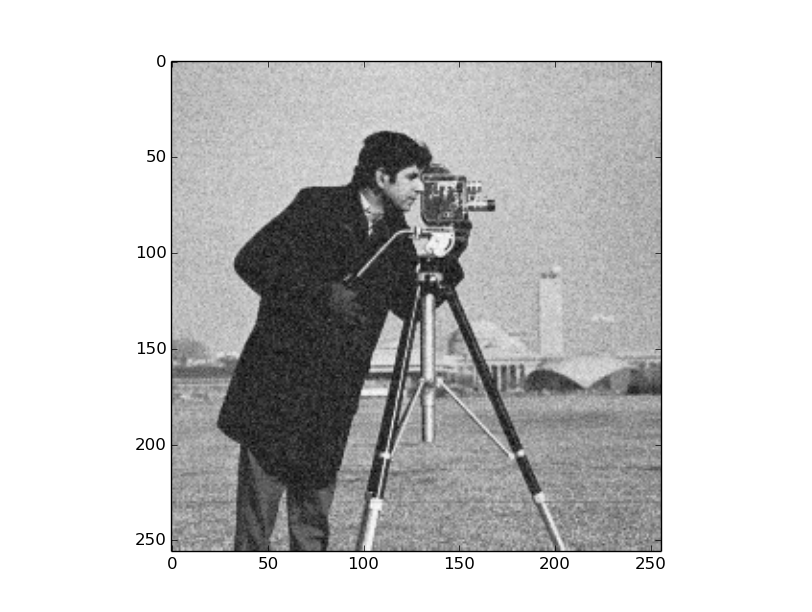
\includegraphics[scale=0.8]{darealest}
\end{figure}
\begin{figure}[H]
  \caption{Billede efter støjreduktion}
  \centering
	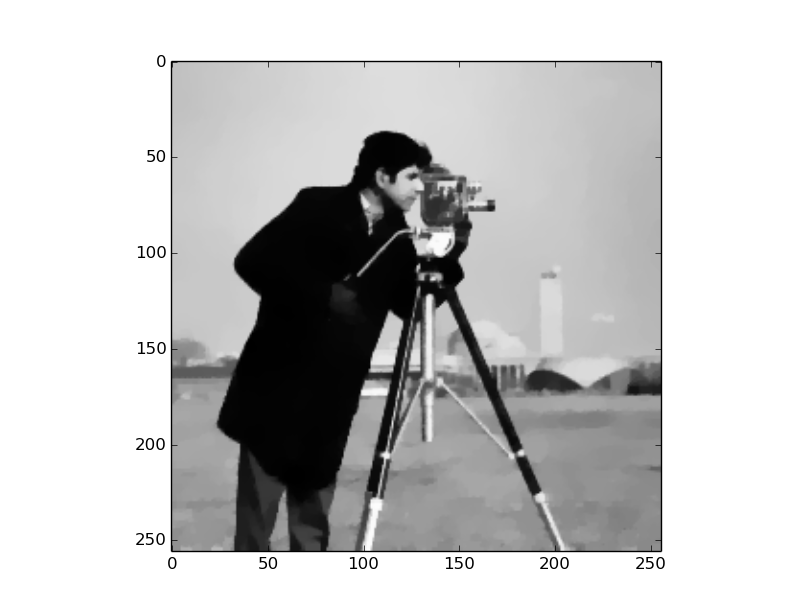
\includegraphics[scale=0.8]{smoothim}
\end{figure}
\end{document}